\documentclass[10pt]{beamer}
\usetheme{Warsaw}
\usepackage[T1]{fontenc}
\usepackage[utf8]{inputenc}
\usepackage{chronosys}
\usepackage{graphicx}
\usepackage{stmaryrd}
\usepackage{float}
\usepackage{caption}
\title{Kinetic}
\author[Demuth Axel, Geraldes Pereira Dorian]{Team member: \newline\newline Demuth Axel \newline Geraldes Pereira Dorian \newline\newline Supervisor :  \newline\newline Pierre Alliez \newline Vincent Chabannes}
\date{}
\begin{document}
\frame{\titlepage}
\begin{frame}
    \tableofcontents
\end{frame}
\section{Introduction}
\begin{frame}{Objectives}
\begin{itemize}
    \item \textbf{Reading Process and Mesh Conversion: }Convert data from stl file to ply and xyz file with normals on points
    
    \item \textbf{Application of the Kinetic Algorithm}
    
    \item \textbf{Recovery of Material Labels}
    
    \item \textbf{Utilization on City Modeling}
\end{itemize}
\end{frame}
\begin{frame}{Challenges}
\begin{itemize}    
    \item \textbf{Generating point cloud from stl file}
\begin{figure}[H]
        \begin{minipage}[t]{0.33\textwidth}
            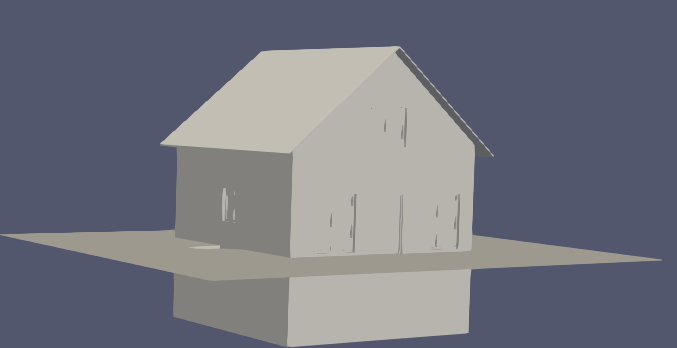
\includegraphics[width=\textwidth]{../../images/screen_kinetic/ACJasmin.png}
            \caption*{ACJasmin stl}
        \end{minipage}
        \begin{minipage}[t]{0.20\textwidth}
          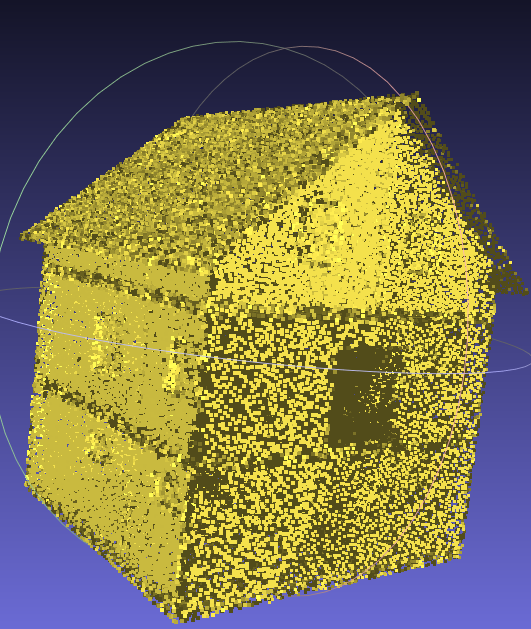
\includegraphics[width=\textwidth]{../../images/screen_kinetic/ACJasmin_point_cloud.png}
          \caption*{ACJasmin point cloud}
        \end{minipage}
\end{figure}
    \item \textbf{Parameter Optimization}
\end{itemize}
\end{frame}

\section{Tools}
\begin{frame}{Cgal}
    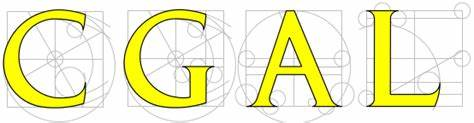
\includegraphics[scale = 0.2]{../../images/CGAL_logo.png}
    \begin{itemize}
        \item C++ library for geometric calcul 
        \item Provides data structures and algorithms for:
        \begin{itemize}
            \item Mesh generation and processing
            \item Geometry processing
            \item Surface and volume manipulation
        \end{itemize}
        \item For our usage Kinetic surface reparation algorithm, filess readers
    \end{itemize}
\end{frame}




\section{Files format}
\begin{frame}{IFC and ply,xyz Files}
\begin{itemize}
    \item IFC : An initiative from buildingSMART (BIM), to standardize files for 3D modeling,similar to  an object-oriented code 
    \item xyz : File format to stock a point cloud
    \item ply : File format to stock a point cloud with normal associated
\end{itemize}


\end{frame}
\begin{frame}{STL (STereoLithography)}
    \begin{itemize}
        \item File format for 3D modeling we convert IFC object to this format
        \item Stock a collection of triangle with normal associated composing  the mesh without any other information
    \end{itemize}
    \begin{center}
        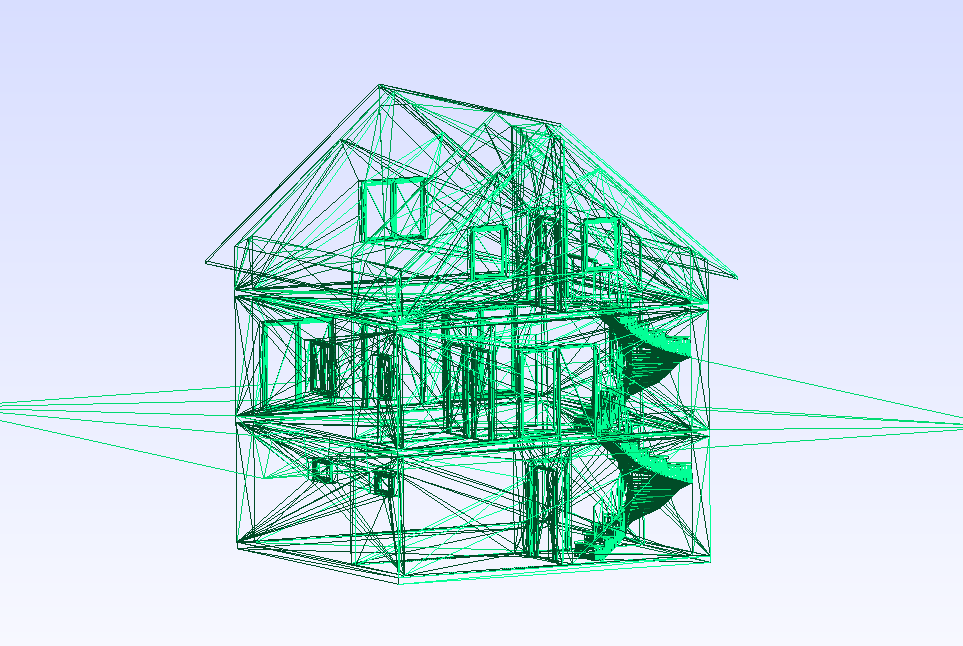
\includegraphics[scale=0.3]{../../images/ACJASMINSTL.png}
    \end{center}
    
\end{frame}

\section{Implementation}
\begin{frame}{Kinetic}
We get information from a INRIA report \cite{yu:hal-03621896}
Kinetic algorithm is an geometric algorithm to work on 3D mesh it uses  geometric primitive with an energy based model to fit the primitives to the model.

Energy formule: 
\newline
\begin{center}
    $        U(x) = w_f U_f(x) + w_s U_s(x) + w_c U_c(x)       $
\end{center}

to calculate the best primitive to fit the mesh.
then we have a list of geometric operation on each primitive
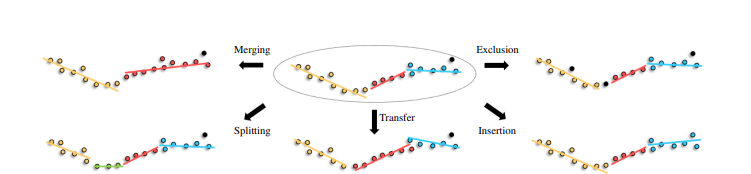
\includegraphics[scale=0.5]{../../images/geometric_operation.png}
\end{frame}
\begin{frame}
    
    Here the speudo code of the application of geometric application : 
    
    \begin{center}
        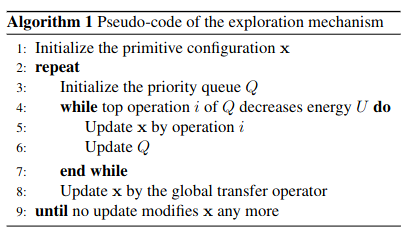
\includegraphics[scale =  0.5]{../../images/Pseudo_code_exploration.png}
      \end{center} 
\end{frame}





\section{Result}
\begin{frame}{first result}
First we can show you what KSR algorithm is capable of: 
\begin{figure}[H]
    \begin{minipage}[t]{0.33\textwidth}
        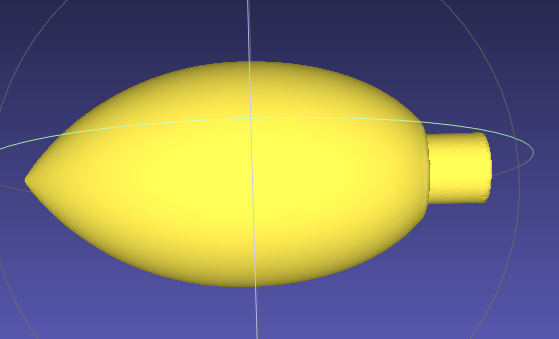
\includegraphics[width=\textwidth]{../../images/screen_kinetic/flame_point.png}
        \caption*{point cloud}
    \end{minipage}
    \begin{minipage}[t]{0.37\textwidth}
      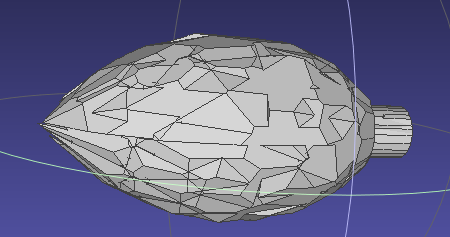
\includegraphics[width=\textwidth]{../../images/screen_kinetic/flame_cgal.png}
      \caption*{cgal result}
    \end{minipage}
    \begin{minipage}[t]{0.32\textwidth}
        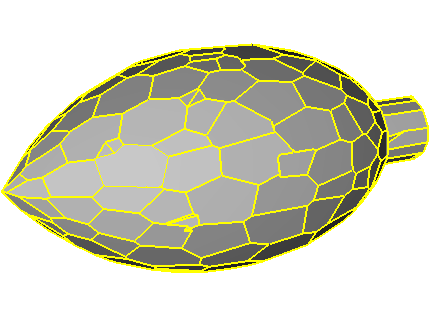
\includegraphics[width=\textwidth]{../../images/screen_kinetic/flame_inria.png}
        \caption*{inria result}
      \end{minipage}
      \caption{Visualization of results on a flame}
\end{figure}
\end{frame}

\begin{frame}{first result}
\begin{figure}[H]
    \centering
    \begin{minipage}[t]{0.35\textwidth}
    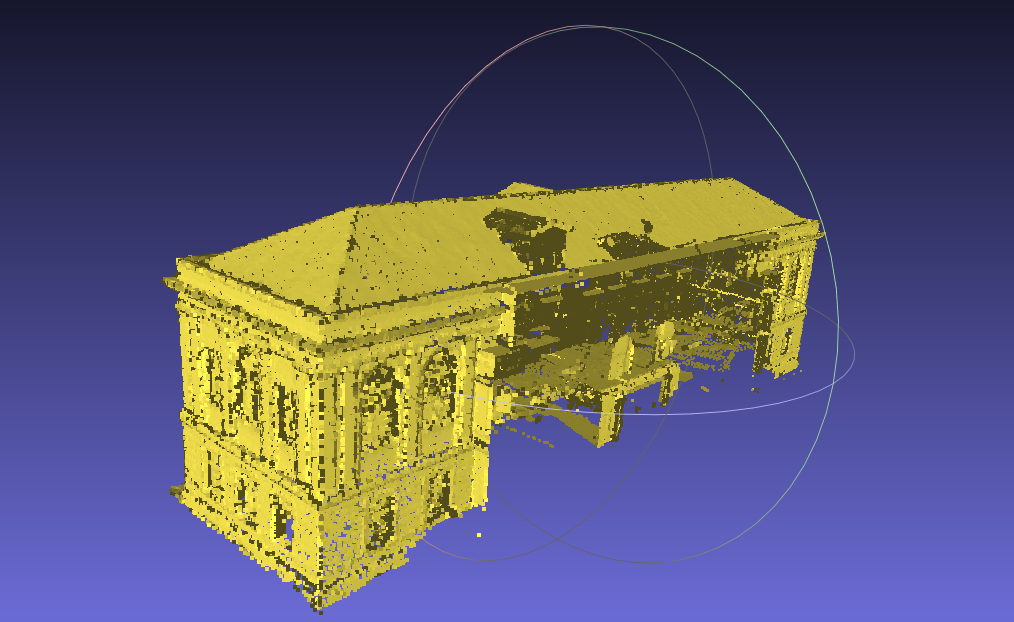
\includegraphics[width=\textwidth]{../../images/screen_kinetic/building_point.png}
    \caption*{point cloud}
\end{minipage}
    \begin{minipage}[t]{0.335\textwidth}
    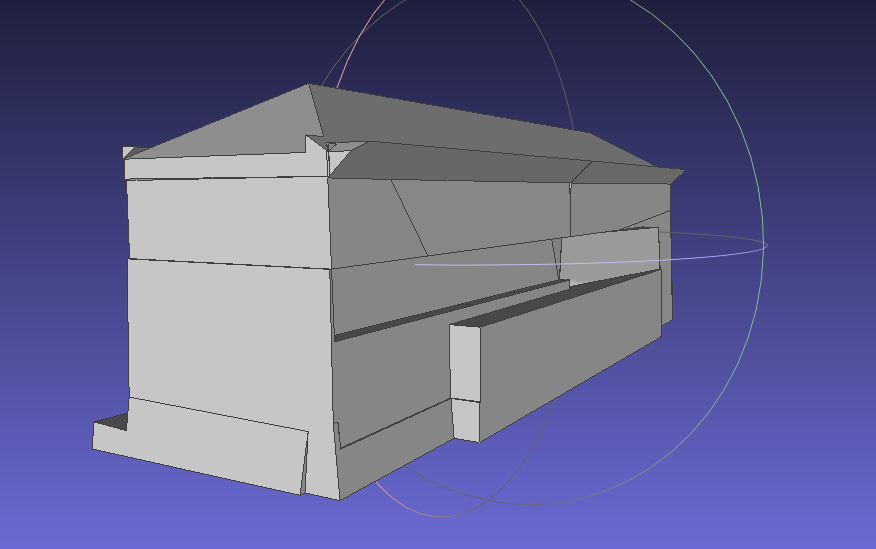
\includegraphics[width=\textwidth]{../../images/screen_kinetic/building_cgal.png}
    \caption*{cgal result}
\end{minipage}
    \begin{minipage}[t]{0.35\textwidth}
    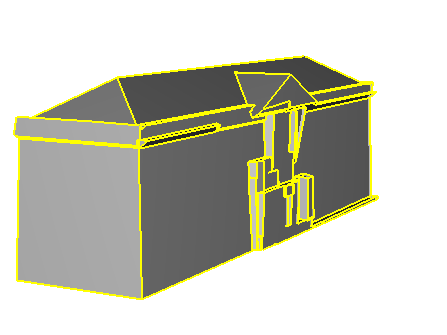
\includegraphics[width=\textwidth]{../../images/screen_kinetic/building_inria.png}
    \caption*{inria result}
    \end{minipage}
    \caption{Visualization of results with a building}
    \end{figure}
\end{frame}
\subsection*{3zones example}
\begin{frame}{3zones example}
    \begin{figure}[H]
        \centering
        \begin{minipage}[t]{0.52\textwidth}
          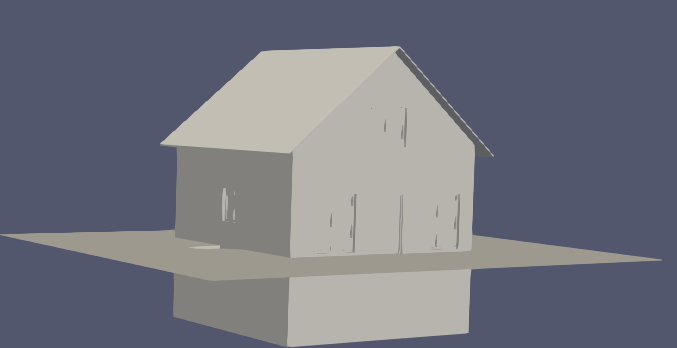
\includegraphics[width=\textwidth]{../../images/screen_kinetic/3zones.png}
          \caption*{3zones}
        \end{minipage}
        \begin{minipage}[t]{0.47\textwidth}
            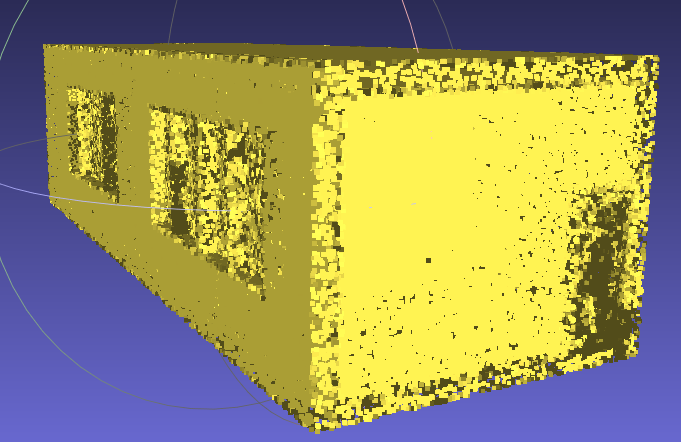
\includegraphics[width=\textwidth]{../../images/screen_kinetic/3zones_point_cloud.png}
            \caption*{3zones point cloud}
          \end{minipage}
        \caption{point cloud conversion}
      \end{figure}  
\end{frame}
\begin{frame}{result}
    \begin{figure}[H]
        \centering
        \begin{minipage}[t]{0.52\textwidth}
          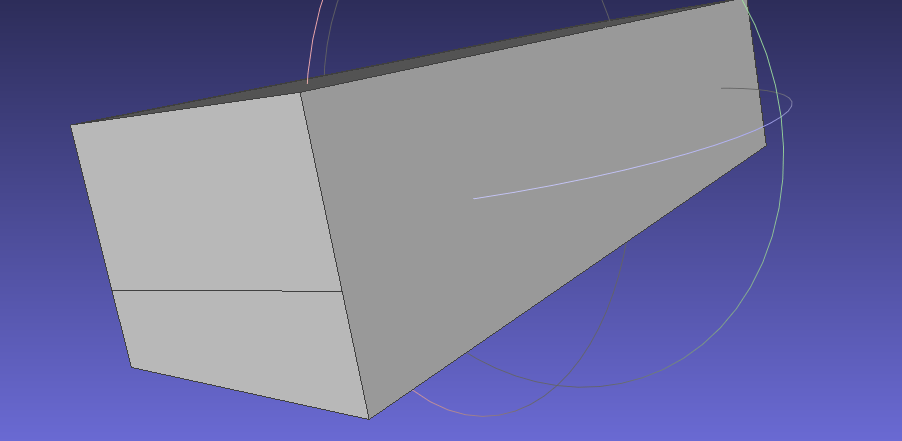
\includegraphics[width=\textwidth]{../../images/screen_kinetic/3zones_result_normal5_cgal.png}
          \caption*{normal by Meshlab}
        \end{minipage}
        \begin{minipage}[t]{0.45\textwidth}
            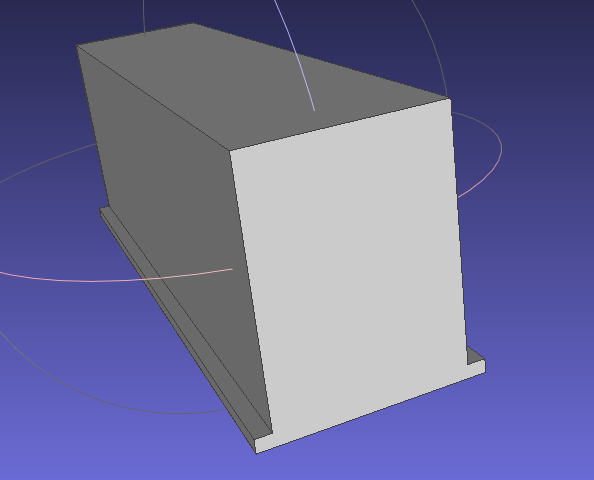
\includegraphics[width=\textwidth]{../../images/screen_kinetic/3zones_result_normal_cgal.png}
            \caption*{normal by Cgal}
          \end{minipage}
        \caption{result on 3zones example}
      \end{figure}  
\end{frame}
\subsection*{ACJasmin example}
\begin{frame}{ACJasmin example }
    \begin{figure}[H]
        \centering
        \begin{minipage}[t]{0.60\textwidth}
          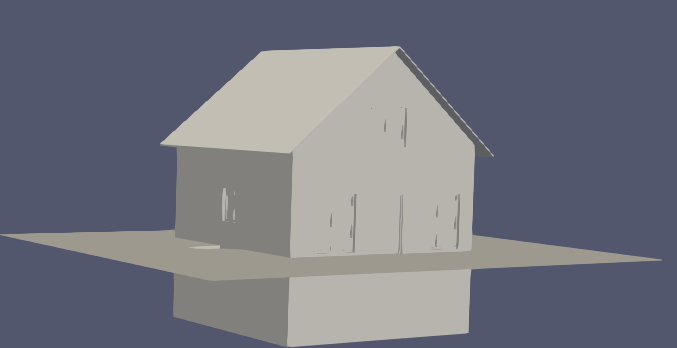
\includegraphics[width=\textwidth]{../../images/screen_kinetic/ACJasmin.png}
          \caption*{ACJasmin}
        \end{minipage}
        \begin{minipage}[t]{0.35\textwidth}
            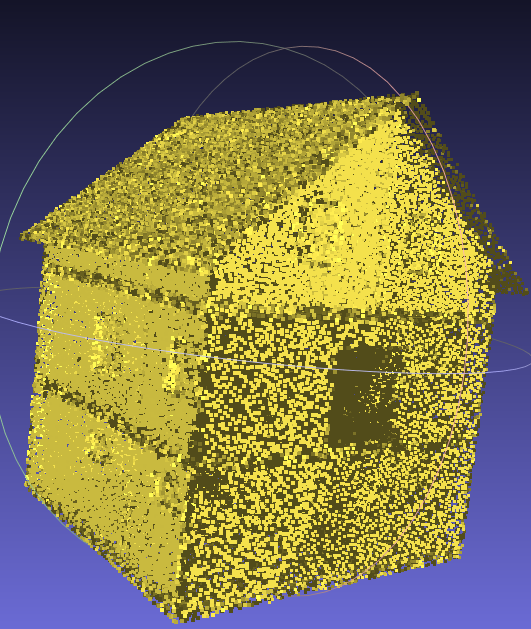
\includegraphics[width=\textwidth]{../../images/screen_kinetic/ACJasmin_point_cloud.png}
            \caption*{ACJasmin point clouds}
          \end{minipage}
          \caption{point cloud conversion}
      \end{figure}  
\end{frame}
\begin{frame}{cgal kinetic result }
    \begin{figure}[H]
        \centering
        \begin{minipage}[t]{0.35\textwidth}
          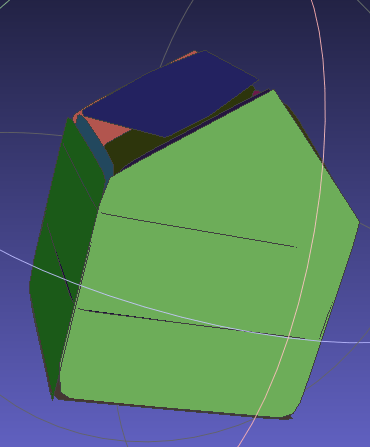
\includegraphics[width=\textwidth]{../../images/screen_kinetic/ACJasmin_primitive_cgal.png}
          \caption*{primitives}
        \end{minipage}
        \begin{minipage}[t]{0.41\textwidth}
            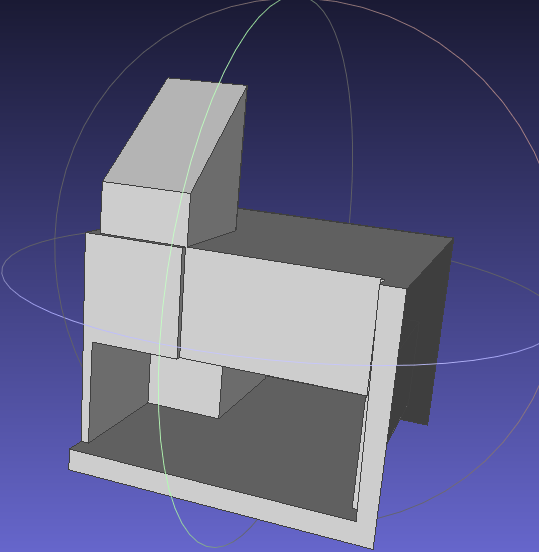
\includegraphics[width=\textwidth]{../../images/screen_kinetic/ACJasmin_result_CGAL.png}
            \caption*{result}
          \end{minipage}
          \caption{result on ACJasmin example using cgal algorithm}
      \end{figure}  
\end{frame}
\begin{frame}{INRIA kinetic result }
    \begin{figure}[H]
        \centering
        \begin{minipage}[t]{0.35\textwidth}
          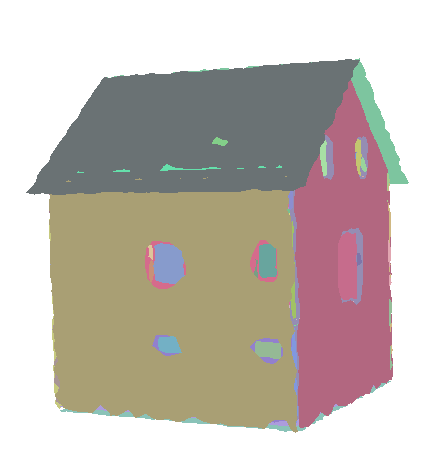
\includegraphics[width=\textwidth]{../../images/screen_kinetic/ACJasmin_primitive.png}
          \caption*{primitives}
        \end{minipage}
        \begin{minipage}[t]{0.35\textwidth}
            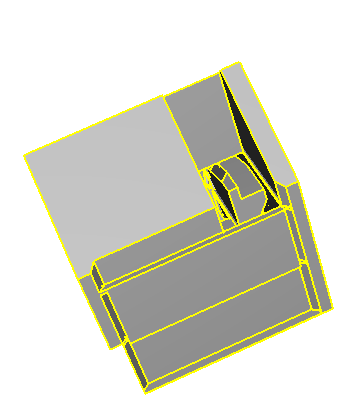
\includegraphics[width=\textwidth]{../../images/screen_kinetic/ACJasmin_result_INRIA.png}
            \caption*{result}
          \end{minipage}
          \caption{result on ACJasmin example using INRIA algorithm}
      \end{figure}  
\end{frame}

\begin{frame}
    Why it does not work? We have few idea  
    \begin{itemize}
        \item Error can be generate when we have not enought point in our point cloud
        \item If the mesh is badly oriented mesh can have problem to generate
    \end{itemize}
\end{frame} 

\begin{frame}{better result }
    \begin{figure}[H]
        \centering
        \begin{minipage}[t]{0.45\textwidth}
          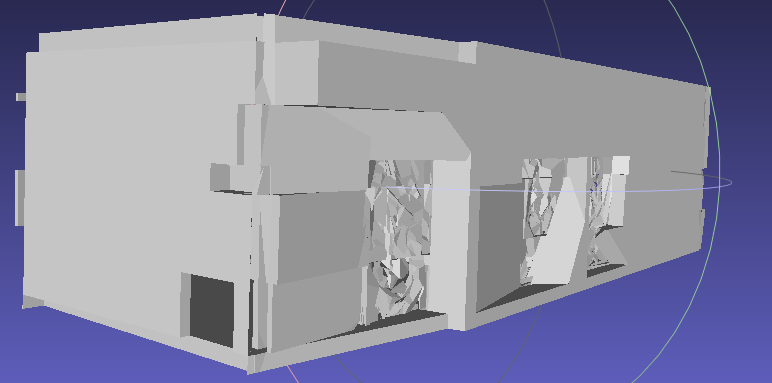
\includegraphics[width=\textwidth]{../../images/screen_kinetic/3zones_v2_1.png}
        \end{minipage}
        \begin{minipage}[t]{0.49\textwidth}
            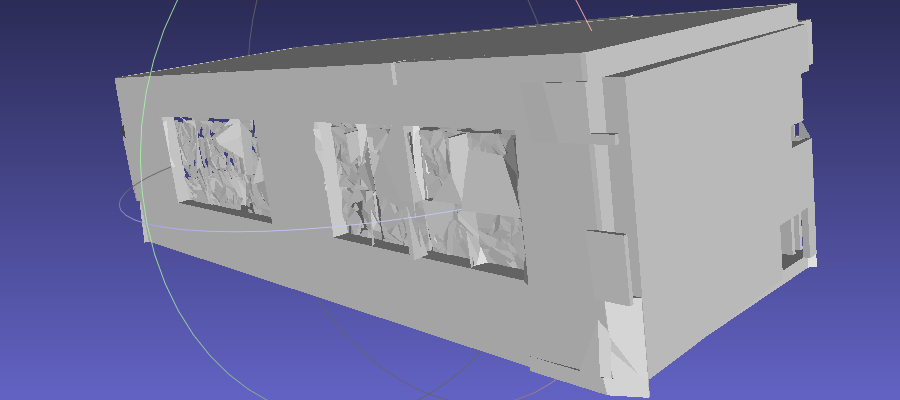
\includegraphics[width=\textwidth]{../../images/screen_kinetic/3zones_v2_2.png}
          \end{minipage}
          \caption{3zones with KSR INRIA, minp=20, epsilon=0.119, Lambda=0 }
      \end{figure}  
\end{frame}


\begin{frame}{Conclusion}
    The kinetic algorithm serves the purpose of upgrading meshes and making them watertight,
    even if some details are lost in the process. However, there are still many limitations regarding its application, and there may be significant preprocessing of the mesh required before executing the algorithm.
\end{frame}


\begin{frame}[allowframebreaks]{reference}
    \nocite{*}
    \bibliographystyle{unsrt}
    \bibliography{../../bibliography/vfinal/report_bib}
\end{frame}

\end{document}